% Robot Perception final project (PPGMC/FURG, 2026/2).
% Every result in the text is a macro from numbers.tex, generated by scripts/06_numbers.py.
% Grey bracketed items are topics for the author to write; they are not part of the paper.
\documentclass[conference]{IEEEtran}
\usepackage{amsmath,amssymb}
\usepackage{graphicx}
\usepackage{booktabs}
\usepackage{cite}
\usepackage{url}
\usepackage{xcolor}
\graphicspath{{figures/}{../figures/}}

% Generated by scripts/06_numbers.py. Do not edit.
\newcommand{\calibRMS}{0.22}
\newcommand{\calibFrames}{156}
\newcommand{\calibFx}{1420.7}
\newcommand{\calibFy}{1420.3}
\newcommand{\calibCx}{631.4}
\newcommand{\calibCy}{468.8}
\newcommand{\calibKone}{0.074}
\newcommand{\calibKtwo}{0.074}
\newcommand{\sigmaMarkerMjpg}{0.09}
\newcommand{\sigmaBoardMjpg}{0.08}
\newcommand{\sigmaMarkerVpeight}{0.13}
\newcommand{\sigmaBoardVpeight}{0.10}
\newcommand{\sigmaEffective}{0.37}
\newcommand{\sigmaFactor}{4.0}
\newcommand{\speedBase}{0.33}
\newcommand{\speedGain}{0.07}
\newcommand{\EoneFrames}{18224}
\newcommand{\EoneBoth}{90.0}
\newcommand{\EoneRot}{0.52}
\newcommand{\EoneTrans}{2.2}
\newcommand{\EoneWrong}{2.6}
\newcommand{\EoneAneesFixed}{680.1}
\newcommand{\EoneMedianFixed}{85.8}
\newcommand{\EoneInsideFixed}{5}
\newcommand{\EoneAneesResidual}{218.0}
\newcommand{\EoneMedianResidual}{76.7}
\newcommand{\EoneInsideResidual}{9}
\newcommand{\EoneAneesEffective}{42.4}
\newcommand{\EoneMedianEffective}{5.3}
\newcommand{\EoneInsideEffective}{70}
\newcommand{\EoneAneesSpeed}{9.2}
\newcommand{\EoneMedianSpeed}{5.3}
\newcommand{\EoneInsideSpeed}{75}
\newcommand{\EfarFrames}{5706}
\newcommand{\EfarBoth}{87.5}
\newcommand{\EfarRot}{2.46}
\newcommand{\EfarTrans}{8.9}
\newcommand{\EfarWrong}{27.9}
\newcommand{\EfarAneesFixed}{825.0}
\newcommand{\EfarMedianFixed}{186.1}
\newcommand{\EfarInsideFixed}{0}
\newcommand{\EfarAneesResidual}{347.6}
\newcommand{\EfarMedianResidual}{74.4}
\newcommand{\EfarInsideResidual}{14}
\newcommand{\EfarAneesEffective}{51.4}
\newcommand{\EfarMedianEffective}{11.6}
\newcommand{\EfarInsideEffective}{54}
\newcommand{\EfarAneesSpeed}{27.6}
\newcommand{\EfarMedianSpeed}{12.1}
\newcommand{\EfarInsideSpeed}{54}
\newcommand{\EtwoFrames}{1158}
\newcommand{\EtwoBoth}{95.8}
\newcommand{\EtwoRot}{0.52}
\newcommand{\EtwoTrans}{1.4}
\newcommand{\EtwoWrong}{0.5}
\newcommand{\EtwoAneesFixed}{214.2}
\newcommand{\EtwoMedianFixed}{97.6}
\newcommand{\EtwoInsideFixed}{1}
\newcommand{\EtwoAneesResidual}{75.2}
\newcommand{\EtwoMedianResidual}{30.9}
\newcommand{\EtwoInsideResidual}{24}
\newcommand{\EtwoAneesEffective}{23.1}
\newcommand{\EtwoMedianEffective}{10.4}
\newcommand{\EtwoInsideEffective}{65}
\newcommand{\EtwoAneesSpeed}{12.1}
\newcommand{\EtwoMedianSpeed}{9.4}
\newcommand{\EtwoInsideSpeed}{72}
\newcommand{\EthreeFrames}{1630}
\newcommand{\EthreeBoth}{85.0}
\newcommand{\EthreeRot}{0.41}
\newcommand{\EthreeTrans}{1.3}
\newcommand{\EthreeWrong}{0.6}
\newcommand{\EthreeAneesFixed}{385.4}
\newcommand{\EthreeMedianFixed}{91.5}
\newcommand{\EthreeInsideFixed}{4}
\newcommand{\EthreeAneesResidual}{61.6}
\newcommand{\EthreeMedianResidual}{16.7}
\newcommand{\EthreeInsideResidual}{45}
\newcommand{\EthreeAneesEffective}{41.7}
\newcommand{\EthreeMedianEffective}{9.9}
\newcommand{\EthreeInsideEffective}{60}
\newcommand{\EthreeAneesSpeed}{19.8}
\newcommand{\EthreeMedianSpeed}{8.2}
\newcommand{\EthreeInsideSpeed}{73}
\newcommand{\EfiveFrames}{1255}
\newcommand{\EfiveBoth}{37.8}
\newcommand{\EfiveRot}{0.31}
\newcommand{\EfiveTrans}{0.9}
\newcommand{\EfiveWrong}{1.5}
\newcommand{\EfiveAneesFixed}{3031.4}
\newcommand{\EfiveMedianFixed}{23.0}
\newcommand{\EfiveInsideFixed}{20}
\newcommand{\EfiveAneesResidual}{22.8}
\newcommand{\EfiveMedianResidual}{12.8}
\newcommand{\EfiveInsideResidual}{57}
\newcommand{\EfiveAneesEffective}{334.1}
\newcommand{\EfiveMedianEffective}{2.6}
\newcommand{\EfiveInsideEffective}{81}
\newcommand{\EfiveAneesSpeed}{145.3}
\newcommand{\EfiveMedianSpeed}{2.9}
\newcommand{\EfiveInsideSpeed}{93}
\newcommand{\occHoldEtwoRot}{7.73}
\newcommand{\occHoldEtwoTrans}{13.1}
\newcommand{\occHoldEtwoLost}{0}
\newcommand{\occHoldEtwoNeesonefive}{2.1}
\newcommand{\occHoldEtwoNeessixonefive}{7.1}
\newcommand{\occHoldEtwoNeesonesixthreezero}{12.2}
\newcommand{\occHoldEtwoNeesthreeonesixzero}{26.3}
\newcommand{\occHoldEthreeRot}{5.15}
\newcommand{\occHoldEthreeTrans}{12.5}
\newcommand{\occHoldEthreeLost}{0}
\newcommand{\occHoldEthreeNeesonefive}{1.4}
\newcommand{\occHoldEthreeNeessixonefive}{4.3}
\newcommand{\occHoldEthreeNeesonesixthreezero}{11.0}
\newcommand{\occHoldEthreeNeesthreeonesixzero}{18.0}
\newcommand{\occHoldEfiveRot}{0.68}
\newcommand{\occHoldEfiveTrans}{4.3}
\newcommand{\occHoldEfiveLost}{0}
\newcommand{\occHoldEfiveNeesonefive}{0.2}
\newcommand{\occHoldEfiveNeessixonefive}{0.2}
\newcommand{\occHoldEfiveNeesonesixthreezero}{0.1}
\newcommand{\occHoldEfiveNeesthreeonesixzero}{0.1}
\newcommand{\occHoldEfiveNeessixoneonezerozerozero}{0.1}
\newcommand{\occRingEtwoRot}{0.76}
\newcommand{\occRingEtwoTrans}{1.8}
\newcommand{\occRingEtwoLost}{32}
\newcommand{\occRingEtwoNeesonefive}{4.3}
\newcommand{\occRingEtwoNeessixonefive}{4.1}
\newcommand{\occRingEtwoNeesonesixthreezero}{3.5}
\newcommand{\occRingEtwoNeesthreeonesixzero}{3.4}
\newcommand{\occRingEthreeRot}{0.64}
\newcommand{\occRingEthreeTrans}{1.4}
\newcommand{\occRingEthreeLost}{29}
\newcommand{\occRingEthreeNeesonefive}{3.2}
\newcommand{\occRingEthreeNeessixonefive}{2.4}
\newcommand{\occRingEthreeNeesonesixthreezero}{2.1}
\newcommand{\occRingEthreeNeesthreeonesixzero}{3.8}
\newcommand{\occRingEfiveRot}{0.43}
\newcommand{\occRingEfiveTrans}{0.8}
\newcommand{\occRingEfiveLost}{16}
\newcommand{\occRingEfiveNeesonefive}{1.1}
\newcommand{\occRingEfiveNeessixonefive}{0.5}
\newcommand{\occRingEfiveNeesonesixthreezero}{0.4}
\newcommand{\occRingEfiveNeesthreeonesixzero}{0.3}
\newcommand{\occRingEfiveNeessixoneonezerozerozero}{0.3}


\newcommand{\topic}[1]{\textcolor{gray}{[#1]}}
\newcommand{\topics}[1]{\begingroup\color{gray}\begin{itemize}#1\end{itemize}\endgroup}
\newcommand{\vect}[1]{\mathbf{#1}}

\begin{document}

\title{Does the Covariance of a Fiducial Marker Pose Match Its Error?\\
A Bench Study for UAV Landing on a Moving Deck}

\author{\IEEEauthorblockN{Aline Timm}
\IEEEauthorblockA{PPGMC, Universidade Federal do Rio Grande (FURG)}}

\maketitle

\begin{abstract}
\topic{150 to 200 words: context, gap, method, result, implication.}
\topics{
\item Context: a UAV landing on a boat needs the pose of the deck and how much to trust it.
\item Gap: marker pipelines give a pose; the precision passed to the decision layer is rarely checked against real error.
\item Method: marker and reference chessboard on one rigid board; first-order covariance; NEES over \EoneFrames{} to \EthreeFrames{} frames per condition; tracking during occlusion.
\item Result: covariance from frame-to-frame noise is inconsistent (median NEES \EtwoMedianFixed{} on E2); a speed-dependent noise model fitted on one video brings it to \EtwoMedianSpeed{}.
\item Implication: the observation precision for the decision layer should grow with target speed.
}
\end{abstract}

\section{Introduction}
\topics{
\item Landing on an unmanned surface vehicle; the deck moves; the thesis uses Active Inference, which needs the precision of each observation.
\item Fiducial markers give pose; the question is whether the covariance they come with matches the error.
\item Why a bench study: ground truth without a simulator, by printing a reference board on the same rigid sheet.
\item Contributions: (1) evaluation of first-order marker covariance against an independent reference with NEES; (2) the finding that error grows with target speed and a noise model that tracks it; (3) tracking through occlusion with growing covariance.
\item Hypotheses H1 to H3 from PLANO.md, stated as tested.
}

\section{Related Work}
Visual landing on a moving platform has been approached with learned and with model-based
pipelines. Polvara et al.~\cite{polvara2018} learn a quadrotor landing policy directly from
low-resolution images of a downward camera, using a hierarchy of deep Q-networks, and evaluate it
in simulated environments with noise. Báča et al.~\cite{baca2019} land a hexacopter on the roof of a
car moving at about 15\,km/h. Their system detects the car with a monocular camera, predicts its
motion and tracks a trajectory from a model predictive controller; it landed three times at the
MBZIRC 2017 competition.
% TODO(Aline): Morales-Rodriguez (2023) from PLANO.md was not found in Crossref or OpenAlex.
% Send its DOI to add it here.

The uncertainty of marker poses has received less attention than their accuracy. Adámek et
al.~\cite{adamek2023} measure the pose estimates of planar fiducial markers in real and simulated 2D
scenes, fit analytical functions to their variance over the measurement range, and use them to fuse
several markers for 2D robot localisation. Our study asks a related question per frame. We take the
first-order covariance that a marker pipeline can compute from its own Jacobian, and test it against
an independent 6-DoF reference with the normalised estimation error squared (NEES).

A square marker seen nearly head-on admits two poses with similar reprojection error. The IPPE
method~\cite{collins2014} returns both, which lets us record how often the chosen one is wrong.

\section{Method}

\subsection{Target, camera and calibration}
The target is one A4 sheet on a rigid wooden board with a chessboard of
$\geoCornersX\times\geoCornersY$ inner corners ($\geoSquare$\,mm squares) and an ArUco marker
(\geoDictionary, $\geoMarker$\,mm). The chessboard is the reference; the marker plays the deck. Poses
map target points to the camera, $\vect{X}_c = \vect{R}\vect{X} + \vect{t}$.

We model the camera as a pinhole with two radial distortion terms. A printed sheet on a board is not
flat, and treating it as flat biases the intrinsics. We therefore estimate the 3D position of every
board corner together with the intrinsics, and then place each marker corner in the target frame by
intersecting the rays from all photos. The photos come from a capture tool that keeps a photo only
when the whole board is visible, sharp and still. Five-fold cross-validation gives the stability of
the intrinsics and the error on photos left out of the fit.

\subsection{Reference and marker poses}
The reference pose $(\vect{R}_b,\vect{t}_b)$ comes from PnP on the $\geoCorners$ board corners with
their measured 3D positions. For a planar target, $(\vect{r}_1,\vect{r}_2,\vect{t})$ and
$(-\vect{r}_1,-\vect{r}_2,-\vect{t})$ give the same image, and the solver sometimes returns the second;
we mirror any solution behind the camera to the front and refine it.

The ArUco detector gives the four marker corners. We refine each one as the intersection of straight
lines fitted to the black-to-white transitions of the two marker edges that meet there, because the
standard sub-pixel refinement targets X-shaped corners and the outer corner of a marker is L-shaped.
IPPE~\cite{collins2014} then gives both marker poses from the measured corner positions; we keep the
one with the lower reprojection error. The pose the marker should have follows from the reference and
the fixed placement $(\vect{R}_{bm},\vect{t}_{bm})$ of the marker on the target,
\begin{equation}
\vect{R}_e = \vect{R}_b\vect{R}_{bm}, \qquad \vect{t}_e = \vect{R}_b\vect{t}_{bm} + \vect{t}_b .
\end{equation}
The error vector $\vect{e} = [\delta\boldsymbol{\theta}^\top, \delta\vect{t}^\top]^\top$ is defined by
\begin{equation}
\vect{R}_m = \exp([\delta\boldsymbol{\theta}]_\times)\,\vect{R}_e, \qquad \vect{t}_m = \vect{t}_e + \delta\vect{t},
\end{equation}
and the rotation error is the geodesic angle $\|\delta\boldsymbol{\theta}\|$.

\subsection{Covariance and consistency}
With $\vect{J}$ the Jacobian of the projected marker corners with respect to the same left
perturbation $[\delta\boldsymbol{\theta}, \delta\vect{t}]$, taken by central differences, and $\sigma$
the corner noise in pixels,
\begin{equation}
\boldsymbol{\Sigma}_m = \sigma^2 (\vect{J}^\top\vect{J})^{-1}.
\end{equation}
The board pose has its own covariance $\boldsymbol{\Sigma}_b$ from its $\geoCorners$ corners, carried to
the expected marker pose by
\begin{equation}
\boldsymbol{\Sigma}_e = \vect{A}\boldsymbol{\Sigma}_b\vect{A}^\top, \quad
\vect{A} = \begin{bmatrix} \vect{I} & \vect{0} \\ -[\vect{R}_b\vect{t}_{bm}]_\times & \vect{I} \end{bmatrix}.
\end{equation}
The NEES of a frame is $\epsilon = \vect{e}^\top(\boldsymbol{\Sigma}_m + \boldsymbol{\Sigma}_e)^{-1}\vect{e}$.
If the covariance is right, $\epsilon$ follows $\chi^2_6$, with mean 6 (the ANEES over frames), median
$\chiMedian$ and 95\% of the frames between $\chiLow$ and $\chiHigh$.

We compare four noise models. (a) Fixed $\sigma$, the corner noise between consecutive frames,
measured on the residual of the marker corners against the prediction from the board in the same
frame; this cancels the motion of the target. (b) Residual $\sigma$ from the frame itself,
$\hat\sigma^2 = \mathrm{RSS}/(8-6)$. (c) Effective $\sigma$, model (a) scaled so that the median NEES of
video E1 equals the $\chi^2_6$ median. (d) Speed $\sigma$,
\begin{equation}
\sigma^2(v) = \sigma_0^2 + (c\,v)^2,
\end{equation}
where $v$ is the mean motion of the marker corners since the previous frame, in pixels per frame. Model
(d) needs neither the board nor future frames, so a landing UAV could use it. Models (c) and (d) are
fitted on E1 alone; every other video is an independent test.

\subsection{Pose during occlusion}
When the marker is not detected, we compare three estimators started from the last frame whose
detection is clean and unambiguous: holding the last pose; Lucas-Kanade tracking of the four marker
corners; and Lucas-Kanade tracking of points on the target around the marker, whose homography from the
start frame carries the four corners along. The region of these ring points excludes the marker and
the chessboard, so the reference never enters the estimate. The tracker declares the target lost when
fewer than 20 points remain, when they cover less than one marker area, or when the corners move more
than three times faster than the marker moved before the loss. After $k$ frames without detection the
covariance grows as
\begin{equation}
\boldsymbol{\Sigma}_k = \boldsymbol{\Sigma} + k\,\vect{Q},
\end{equation}
with a diagonal $\vect{Q}$ fitted, per estimator, on half of the synthetic occlusions of E2 from the
median squared error in bins of $k$.

\section{Experimental Setup}
The camera is a fixed-focus webcam at $\camWidth\times\camHeight$ pixels and 30 frames per second, with
exposure, gain and white balance locked. Calibration used $\calibPhotos$ photos, of which
$\calibFrames$ with distinct poses entered the fit. Fig.~\ref{fig:setup} shows the target and
Fig.~\ref{fig:pipeline} the pipeline.

Table~\ref{tab:protocol} lists the recordings. In E1 the board stood on a chair and the camera moved
between still poses, because a hand-held board drifted by more than three pixels within seconds. E2,
E3 and E5 were hand-held and compressed by the recording application with the VP8 codec; E1 keeps the
JPEG of each camera frame. A glare condition was planned with a plastic film over the target and was
dropped, because the film prevented the detection of the reference. For the occlusion study we painted
a grey patch over the marker in E2 and E3 for windows of 15, 30 and 60 frames, $\occWindows$ windows in
all, leaving the board visible. E5 holds $\occReal$ real occlusions by a hand.

\begin{table}[t]
\caption{Recordings. All at $\camWidth\times\camHeight$ pixels.}
\label{tab:protocol}
\centering
\begin{tabular}{llr}
\toprule
ID & Content & Frames \\
\midrule
E1 & Still poses, board on a chair & \EoneFrames \\
Far & Still, frontal, $\EfarDistance$\,m & \EfarFrames \\
E2 & Slow rocking by hand & \EtwoFrames \\
E3 & Strong tilts and frontal passes & \EthreeFrames \\
E5 & Marker covered by a hand & \EfiveFrames \\
\bottomrule
\end{tabular}
\end{table}

\section{Results}

\subsection{Calibration}
The fit reached an RMS reprojection error of $\calibRMS$\,px, and $\calibHeldLow$ to $\calibHeldHigh$\,px on
photos left out of it. Across the five folds the focal length varied by $\calibSdFocal$\,px (standard
deviation) and the principal point by $\calibSdCentre$\,px. The sheet departs from a plane by up to
$\calibBend$\,mm. Predicting the marker corners from the board pose gives $\calibMarkerNominal$\,px of
error with the printed marker position and $\calibMarkerMeasured$\,px with the measured one, whose
corners sit $\calibShiftLow$ to $\calibShiftHigh$\,mm from the printed design.

\subsection{Error and consistency}
Table~\ref{tab:results} summarises each condition. In E2 the median marker error is $\EtwoRot$\,deg and
$\EtwoTrans$\,mm. With fixed noise ($\sigma = \sigmaMarkerMjpg$\,px for E1,
$\sigmaMarkerVpeight$\,px for the VP8 videos), the NEES is far above its expected value in every
condition, with a median of $\EtwoMedianFixed$ in E2 and $\EthreeMedianFixed$ in E3 against $\chiMedian$.
Fig.~\ref{fig:time} shows why. The error moves well outside the $\pm2\sigma$ band of fixed noise, mostly
where the board moves. Residual noise, model (b), does not change this (Fig.~\ref{fig:nees}).

The effective model needs $\sigma = \sigmaEffective$\,px, $\sigmaFactor$ times the noise between frames.
On the independent videos its median NEES is $\EtwoMedianEffective$ (E2) and $\EthreeMedianEffective$
(E3). The speed model fitted on E1 gives $\sigma_0 = \speedBase$\,px and $c = \speedGain$, and median NEES
of $\EtwoMedianSpeed$ and $\EthreeMedianSpeed$, with $\EtwoInsideSpeed$\% and $\EthreeInsideSpeed$\% of the
frames inside the 95\% interval. Its ANEES stays above 6 ($\EtwoAneesSpeed$ and $\EthreeAneesSpeed$).
Fig.~\ref{fig:speed} explains the gain. Above 10\,px per frame the median NEES of E3 is
$\EthreeSpeedEFixed$ with fixed noise, $\EthreeSpeedEEffective$ with effective noise and
$\EthreeSpeedESpeed$ with speed noise. Below 0.3\,px per frame it is $\EthreeSpeedASpeed$.

These observations suggest that most of the error the covariance misses comes with motion. The noise
measured between frames leaves out what happens to the corners when the marker moves during the exposure.

\subsection{Tilt and ambiguity}
The rotation error falls with tilt (Fig.~\ref{fig:tilt}a). In E3 its median goes from $\EthreeTiltARot$\,deg
below 15\,deg of tilt to $\EthreeTiltERot$\,deg above 60\,deg, over $\EthreeTiltEFrames$ frames. The wrong
IPPE solution is chosen in $\EoneTiltAWrong$\% of the E1 frames below 15\,deg and in $\EfarTiltAWrong$\% of
the frontal frames at $\EfarDistance$\,m. The median NEES of the speed model does not grow above 60\,deg
(Fig.~\ref{fig:tilt}b). In E2 and E3 it is highest at intermediate tilts.

\subsection{Occlusion}
Holding the last pose gives a median error of $\occHoldEtwoRot$\,deg and $\occHoldEtwoTrans$\,mm over
the E2 test windows. Ring tracking gives $\occRingEtwoRot$\,deg and $\occRingEtwoTrans$\,mm, and loses
the target in $\occRingEtwoLost$\% of the frames. Tracking the four corners, the method we planned, loses
$\occCornersEtwoLost$\% of the frames under a full cover (Fig.~\ref{fig:occlusion}).

For ring tracking, the error grows slowly with $k$. The median is $\occRingEtwoKARot$\,deg and
$\occRingEtwoKATrans$\,mm in the first five frames and $\occRingEtwoKBRot$\,deg and $\occRingEtwoKBTrans$\,mm
from 6 to 15 frames. The median NEES with $\boldsymbol{\Sigma}_k$ stays near the $\chi^2_6$ median
($\occRingEtwoKANees$ and $\occRingEtwoKBNees$) with $\occRingEtwoKAInside$\% and $\occRingEtwoKBInside$\% of
the frames inside the interval. Beyond 30 frames, $\occRingEtwoKDLost$\% of the tracks are lost. On the
real occlusions of E5 the median error is $\occRingEfiveRot$\,deg and $\occRingEfiveTrans$\,mm.

\begin{table*}[t]
\caption{Marker error and consistency per condition. ANEES should be 6 and 95\% of the frames should
fall inside the $\chi^2_6$ interval. E1 is the fit set of the speed model.}
\label{tab:results}
\centering
% Generated by scripts/06_numbers.py. Do not edit.
\begin{tabular}{lrrrrrrrr}
\toprule
 & & & \multicolumn{2}{c}{Median error} & \multicolumn{2}{c}{Fixed $\sigma$} & \multicolumn{2}{c}{Speed $\sigma$} \\
Condition & Frames & Detected (\%) & deg & mm & ANEES & In 95\% & ANEES & In 95\% \\
\midrule
E1 (fit) & 18224 & 90.0 & 0.52 & 2.2 & 680 & 5 & 9.2 & 75 \\
Far, 1.66 m & 5706 & 87.5 & 2.46 & 8.9 & 825 & 0 & 27.6 & 54 \\
E2 & 1158 & 95.8 & 0.52 & 1.4 & 214 & 1 & 12.1 & 72 \\
E3 & 1630 & 85.0 & 0.41 & 1.3 & 385 & 4 & 19.8 & 73 \\
E5 & 1255 & 37.8 & 0.31 & 0.9 & 3031 & 20 & 145.3 & 93 \\
\bottomrule
\end{tabular}

\end{table*}

\section{Discussion}
\topics{
\item H1 refuted as stated: with the noise between frames the covariance is optimistic by about $\sigmaFactor$ in standard deviation. Say how this compares with the variance models of~\cite{adamek2023}.
\item What the speed model fixes and what it does not: the median becomes plausible, the ANEES stays above 6, carried by few frames.
\item H2 in two parts: ambiguity near frontal confirmed, worse at distance; no degradation above 60 degrees, against the hypothesis.
\item H3: ring tracking usable for about half a second; long tracks get lost; the corner tracking of the plan does not work under a full cover.
\item Possible causes of the motion error, not tested: rolling shutter, motion blur, compression; the position in the image mattered little.
\item Limits of the bench: hand-held motion, no water, no glare (E4 dropped), one camera, a target that is not flat and had to be measured.
\item What the thesis gets: an observation precision that grows with speed and with time without detection.
}

\section{Conclusion}
\topics{
\item Two or three sentences: question, main answer, what changes for the landing controller.
\item Future work: Gazebo, field videos from the Hydrone, other cameras, a cause for the motion error.
}

\section*{Acknowledgment}
\topic{Check against the course policy on LLM use and edit.} This work used an LLM assistant (Claude,
Anthropic) to write and test the analysis code and to draft the Method, Experimental Setup and Results
sections. The author checked the code, the figures and every statement of the paper.

\bibliographystyle{IEEEtran}
\bibliography{refs}

% Figures are placed at the end of the source; LaTeX floats them near their first mention.
\begin{figure}[t]
\centering
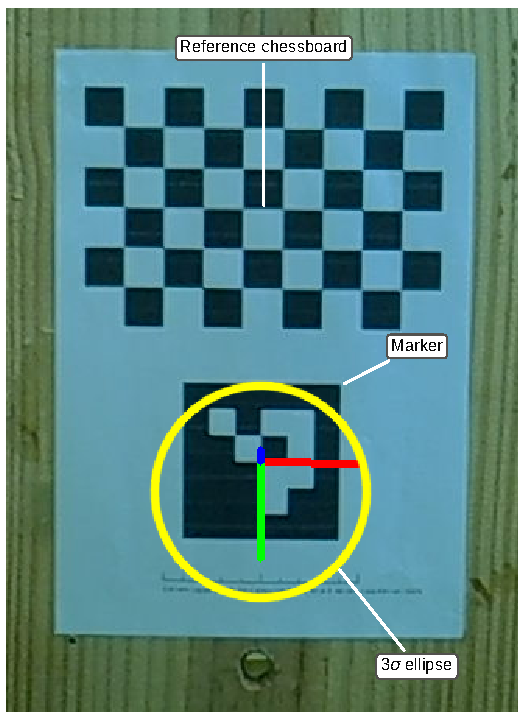
\includegraphics[width=\columnwidth]{fig1_setup}
\caption{Target on its board: reference chessboard, marker with its axes and the 3$\sigma$ ellipse of
the tip of its normal (100\,mm long, ellipse enlarged five times for visibility).}
\label{fig:setup}
\end{figure}

\begin{figure*}[t]
\centering
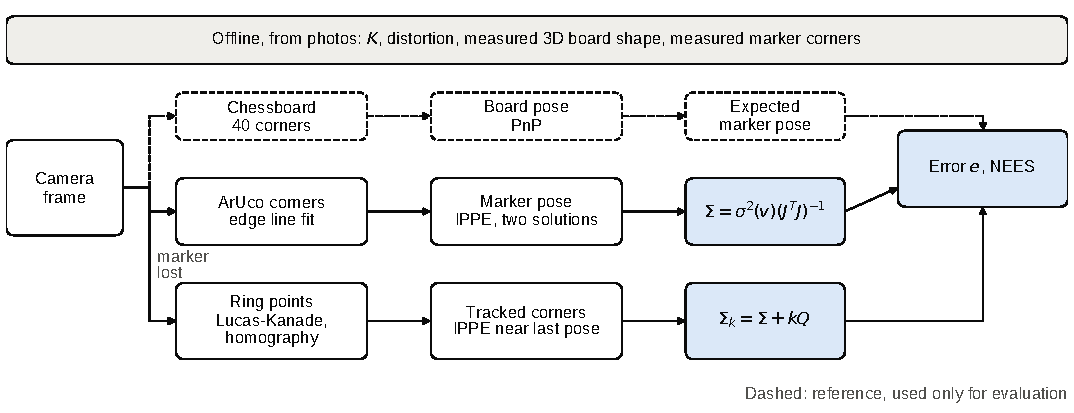
\includegraphics[width=\textwidth]{fig2_pipeline}
\caption{Pipeline. The chessboard path (dashed) only measures the error; the marker pose and its
covariance never use it.}
\label{fig:pipeline}
\end{figure*}

\begin{figure*}[t]
\centering
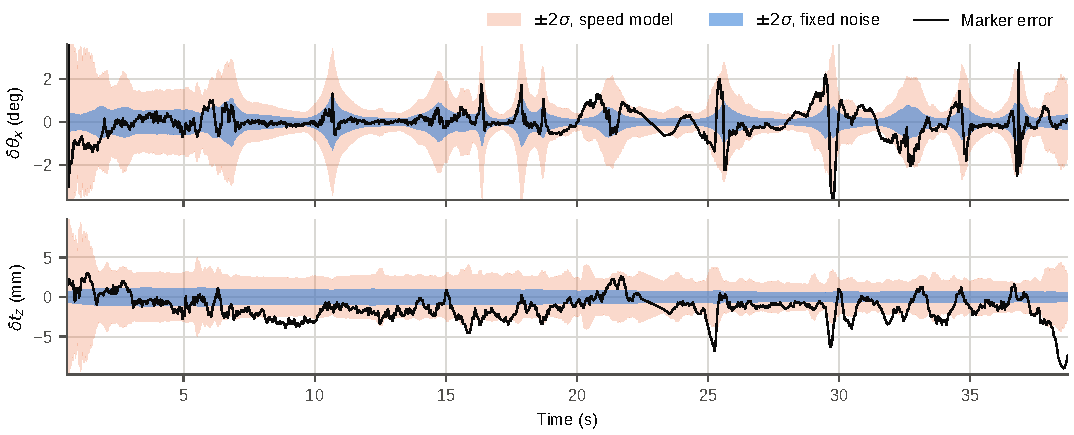
\includegraphics[width=\textwidth]{fig3_error_time}
\caption{Marker error in E2 for one rotation and one translation component, with the $\pm2\sigma$
bands of the fixed and speed noise models. The vertical axes are cut at 1.15 times the 99.5th
percentile of the error, which clips the first second.}
\label{fig:time}
\end{figure*}

\begin{figure*}[t]
\centering
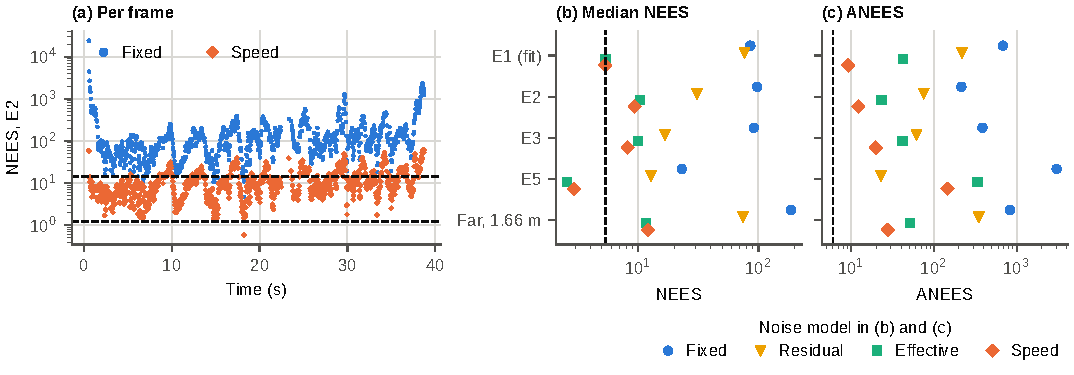
\includegraphics[width=\textwidth]{fig4_nees}
\caption{(a) NEES per frame in E2. (b) Median NEES and (c) ANEES per condition and noise model. Dashed
lines: the $\chi^2_6$ 95\% interval in (a), its median in (b) and its mean in (c).}
\label{fig:nees}
\end{figure*}

\begin{figure*}[t]
\centering
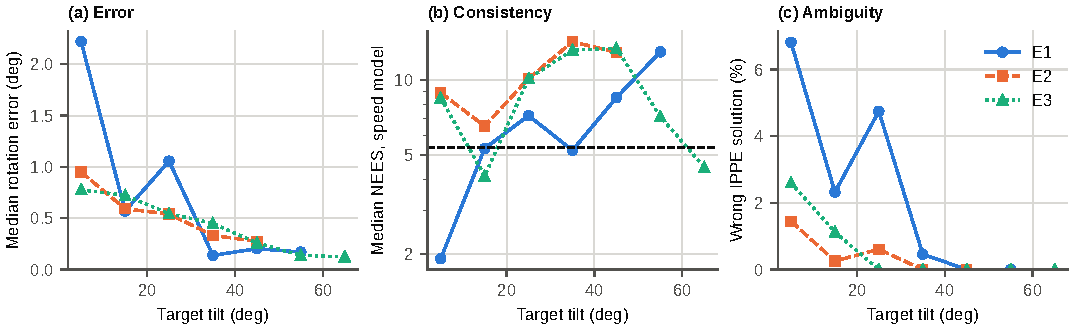
\includegraphics[width=\textwidth]{fig5_tilt}
\caption{Effect of the tilt of the target, in bins of 10\,deg with at least 30 frames. (a) Median rotation
error. (b) Median NEES with the speed model; dashed, the $\chi^2_6$ median. (c) Frames where the other IPPE
solution was closer to the reference.}
\label{fig:tilt}
\end{figure*}

\begin{figure*}[t]
\centering
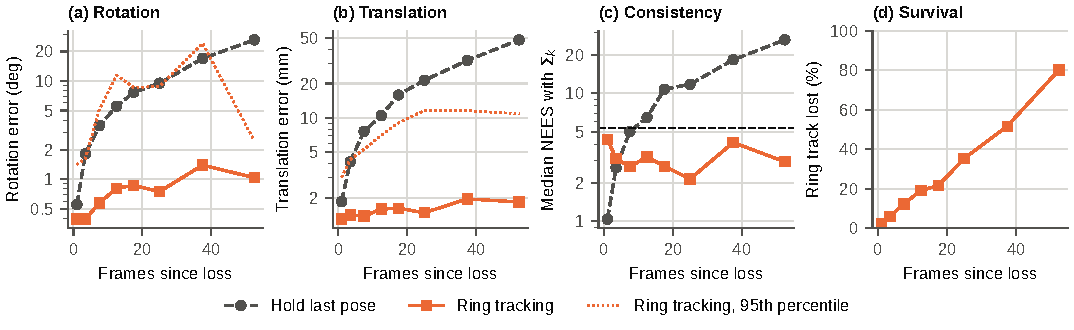
\includegraphics[width=\textwidth]{fig6_occlusion}
\caption{Synthetic occlusions of E2 (test windows) and E3, against the frames since the marker was
lost. Medians over the tracks still alive; the 95th percentile drops after 30 frames because the tracks
with large errors were already lost, not because the tracking improves.}
\label{fig:occlusion}
\end{figure*}

\begin{figure}[t]
\centering
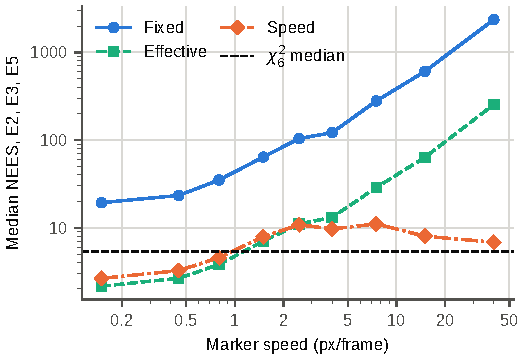
\includegraphics[width=\columnwidth]{fig7_speed}
\caption{Median NEES against the speed of the marker in the independent videos E2, E3 and E5.}
\label{fig:speed}
\end{figure}

\end{document}
